%% ICAIF submission — ACM sigconf.
%% Toggle `anonymous` for double-blind review (confirm ICAIF policy before submitting).
\documentclass[sigconf,nonacm]{acmart}
%% For camera-ready with ACM reference, remove `nonacm` and fill in the rights block.

\settopmatter{printacmref=false}
\setcopyright{none}
\renewcommand\footnotetextcopyrightpermission[1]{}
\pagestyle{plain}

\usepackage{booktabs}
\usepackage{amsmath}
\usepackage{graphicx}
\usepackage{xcolor}
\usepackage{subcaption}

% draft helpers (strip before submission)
\newcommand{\todo}[1]{\textcolor{red}{[TODO: #1]}}
\newcommand{\num}[1]{#1}   % wrap final numbers so they are easy to grep/update

\begin{document}

\title{When Two Attentions Aren't Enough: Count- and Pattern-Aware
Cross-Sequence Encoding for Relational Fraud in Financial Foundation Models}

\author{Anonymous Author(s)}
\affiliation{\institution{Anonymous Institution}\country{}}

\begin{abstract}
Financial foundation models (FFMs) --- masked-pretrained, encoder-only transformers over
per-account event sequences, adapted with a lightweight head --- have been proposed to
replace the hand-engineered features and gradient-boosted decision trees (GBDTs) that
dominate production fraud detection. Such models use \emph{two} attentions: one over the
fields of an event, and one over an account's own event history. We show this design is
\emph{structurally blind} to \emph{relational} fraud --- patterns that live in a shared
entity's activity \emph{across} accounts (a compromised merchant hit by many cards; a
fraud-farm IP driving many devices) --- which no per-account model can see. We add a
\emph{third}, cross-sequence attention and study when it helps. On a controlled synthetic
benchmark with ground-truth signal placement, a per-account FFM collapses to the base rate
on relational fraud while the cross-sequence encoder recovers it. Across four real datasets
we then map \emph{when} it helps: the relational signal is sometimes a \emph{pattern} in a
neighbour's raw events (where attention over neighbours wins) and sometimes a \emph{count}
--- a velocity magnitude a scalar aggregate captures losslessly but a bounded attention
window truncates. We reconcile the two with a \emph{count-aware} cross-sequence encoder that
carries both a raw-neighbour attention path and a log-count magnitude readout. A single such
module is the best arm in \emph{both} regimes over three seeds: on real click fraud (TalkingData)
it beats the per-account FFM by \num{+0.084} PR-AUC ($0.700\pm0.011$ vs.\ $0.616\pm0.013$), and on
the synthetic benchmark it \emph{stabilises} an otherwise wildly seed-unstable raw-attention arm
($0.318\pm0.010$ vs.\ $0.252\pm0.117$). We close with the productization
levers this enables --- neighbour-embedding caching for a frozen backbone, and the count vs.\
pattern taxonomy that tells practitioners which relational encoder a given fraud problem
needs.

\end{abstract}

\keywords{financial foundation models, fraud detection, event-sequence
transformers, relational learning, gradient-boosted trees}

\maketitle

\section{Introduction}

Fraud detection and related risk tasks at scale are still dominated by gradient-boosted decision
trees (GBDTs) over hand-engineered features~\cite{ke2017lightgbm,chen2016xgboost}. A compelling
alternative, mirroring foundation models elsewhere~\cite{bommasani2021foundation}, is to pretrain a
transformer on raw event sequences with a self-supervised objective and adapt it to downstream tasks
with a lightweight head --- a \emph{financial foundation model}
(FFM)~\cite{ostroukhov2026pragma,yeh2025treasure,padhi2021tabular}. Each transaction is tokenised
into field--value tokens; a set transformer encodes the fields of an event, and a temporal
transformer encodes an account's history of such events; adaptation reads the final-position
embedding with a linear probe or a light fine-tune.

In effect these models use \emph{two attentions}: one \emph{within} an event, over its fields, and
one \emph{across} an account's own history. Our observation is that this design sees only one entity
in isolation and is therefore \textbf{structurally blind to relational signal} --- patterns that
live in a shared entity's activity \emph{across} accounts. A compromised merchant produces a burst
of fraud spread over many cards; a fraud-farm IP drives many devices; a product goes viral across
many shoppers. None of these are visible to a model that attends only within a single account's
sequence, no matter how it is trained.

We add a \emph{third}, \textbf{cross-sequence attention}: for a target event at a shared entity
(merchant, IP, item, \dots), the model attends over that entity's recent events from \emph{other}
sequences, encoded by the same event encoder. Crucially we add it at \emph{fine-tuning time}, on top
of a pretrained two-attention backbone, rather than changing the pretraining recipe. This keeps the
FFM intact and makes the module a drop-in adaptation choice.

Our contributions are:
\begin{itemize}
\item \textbf{A third attention for FFMs (\S\ref{sec:method}).} A cross-sequence encoder that lets a
target event attend over a shared entity's recent cross-account events, added at fine-tuning time
and trained end-to-end with a linear head.
\item \textbf{Consistent relational gains (\S\ref{sec:results}).} Across three datasets where a
relational signal exists, the third attention improves \prauc{} by \num{+0.04} to \num{+0.07} over
standard fine-tuning of the same backbone.
\item \textbf{An isolation control.} On a synthetic benchmark with \emph{no} relational signal, the
gain \emph{collapses to zero} --- the same added capacity yields nothing --- establishing that the
improvement is the cross-sequence signal, not extra parameters.
\item \textbf{Beating a strong tabular baseline, and generalisation beyond fraud.} On TalkingData
the fine-tuned FFM with the third attention exceeds a strong GBDT; and on a non-fraud e-commerce
conversion task (Retailrocket) the same module delivers the same relational lift, showing the idea
is not fraud-specific.
\end{itemize}

All code, the synthetic generator, dataset adapters, and per-experiment result files are released for
reproducibility.

\section{Background and related work}

\paragraph{Event-sequence and tabular transformers.} Encoder-only, masked-pretrained
transformers~\cite{vaswani2017attention,devlin2019bert} over tokenised tabular/event sequences
are established: BEHRT for medical records~\cite{li2020behrt} and
TabBERT/TabFormer for transactions~\cite{padhi2021tabular} introduced the hierarchical
field-then-sequence design our FFM follows, related tabular transformers add contextual and
row-attention encodings~\cite{huang2020tabtransformer,somepalli2021saint}, and later work
studied numeric encodings (piecewise-linear, periodic)~\cite{gorishniy2022embeddings}.
Industrial financial foundation models scale this recipe to billions of banking
events~\cite{braithwaite2025spending}; we discuss the two closest to our setting below. The neural
\emph{architecture} we build on is therefore not itself novel; our object of study is the
\emph{transfer} recipe (pretrain once, adapt with a light head) and, specifically, what it misses
relationally.

\paragraph{Industrial FFMs and the relational gap.} Two recent industrial systems make the FFM
recipe concrete at scale, and are the closest prior work to ours. PRAGMA~\cite{ostroukhov2026pragma}
pre-trains a masked transformer on heterogeneous, multi-source banking event sequences and serves
credit scoring, fraud, and lifetime-value prediction from one representation read by a linear probe
or a lightweight fine-tune --- the exact recipe we reproduce at laptop scale. TREASURE~\cite{yeh2025treasure}
encodes payment-network transactions with dedicated static- and dynamic-attribute modules and,
notably, ingests \emph{payment-network signals} (response codes, system flags) alongside consumer
behaviour, reporting large gains on abnormal-behaviour detection. Both establish the value of the
pretrain-once, adapt-lightly recipe on real financial data at industrial scale. Crucially, however,
each encodes a \emph{single entity's own event stream}: PRAGMA a user's banking history, TREASURE a
consumer's transactions --- and the network signals TREASURE reads are attributes \emph{recorded on
that consumer's own events}, not the concurrent activity of a shared merchant or IP across
\emph{other} consumers. This is precisely the structural blindness we target: the signal in a
compromised merchant or a fraud-farm IP lives in \emph{concurrent, cross-account} activity that no
per-entity encoder observes at inference. Our cross-sequence attention is therefore
\emph{orthogonal and composable} --- it augments rather than replaces a PRAGMA- or TREASURE-style
backbone, adding a third attention over a shared entity's events from other accounts while leaving
the per-entity encoders and the pretraining recipe intact.

\paragraph{Generative recommender foundation models.} Per-user sequence transformers underpin
sequential recommendation~\cite{kang2018sasrec,sun2019bert4rec}, and HSTU, OneRec, and
TIGER~\cite{zhai2024hstu,deng2024onerec,rajput2023tiger} reformulate
recommendation as sequential transduction over a user's interactions and scale to enormous sizes.
These are architecturally the same per-user sequence transformers, yet highly effective, for two
reasons we make precise: their pretraining objective \emph{is} the downstream task (next item) and
they train end-to-end (no proxy, no frozen bottleneck), and the relational signal they rely on
(collaborative affinities) is largely \emph{stationary} and absorbs into shared item embeddings ---
unlike the \emph{transient} cross-entity state (``compromised right now'') that characterises much
fraud, which must be read from concurrent cross-sequence activity.

\paragraph{GBDTs and graph methods for fraud.} Gradient-boosted trees~\cite{ke2017lightgbm,chen2016xgboost}
with client- and entity-level aggregates remain the production and competition standard. On graph
fraud, methods such as CARE-GNN and PC-GNN~\cite{dou2020caregnn,liu2021pcgnn} beat plain GNNs by
\emph{similarity-based neighbour selection} to
resist \emph{camouflage} (fraud nodes wiring mostly to legitimate ones); we return to this when we
find plain neighbour attention underperforms on camouflaged graphs (\S\ref{sec:boundary}). Our
contribution is orthogonal: a sequence-native cross-sequence attention for FFMs, and a map of when
it beats a scalar aggregate.

\section{Method}
\label{sec:method}

% Three-attentions schematic. Compiles with tikz (verify on first build).
\begin{figure}[t]
\centering
\begin{tikzpicture}[
  font=\small,
  box/.style={draw, rounded corners, minimum height=7mm, align=center, inner sep=3pt},
  enc/.style={box, fill=blue!8},
  att/.style={box, fill=orange!12},
  ar/.style={-{Latex[length=2mm]}, thick},
  node distance=5mm and 7mm]

\node[box, fill=gray!8] (fields) {event\\fields};
\node[enc, right=of fields] (evt) {Event\\Encoder\\{\scriptsize(attn 1)}};
\node[att, right=of evt] (hist) {History\\Encoder\\{\scriptsize(attn 2)}};
\node[box, right=of hist, fill=green!8] (head) {head};
\node[right=4mm of head] (out) {$\hat{y}$};

\draw[ar] (fields) -- (evt);
\draw[ar] (evt) -- (hist) node[midway,above,font=\scriptsize] {[EVT]};
\draw[ar] (hist) -- (head) node[midway,above,font=\scriptsize] {record emb.};
\draw[ar] (head) -- (out);

% cross-sequence (third attention) below
\node[box, fill=gray!8, below=9mm of evt] (nbr) {last-$K$ neighbour\\events at shared\\entity (other accts.)};
\node[att, right=of nbr, minimum height=10mm] (xseq)
  {Cross-Sequence Encoder\\{\scriptsize the third attention (attn 3)}};
\draw[ar] (nbr) -- (xseq);
\draw[ar, dashed] (nbr.north) to[out=90,in=180] (evt.west|-nbr.north) ;
\draw[ar] (evt.south) to[out=-90,in=180] ([yshift=2mm]xseq.west);
\draw[ar] (xseq.north) to[out=90,in=-90] (hist.south)
  node[midway,right,font=\scriptsize] {$+$ residual};

\begin{scope}[on background layer]
\node[draw, dotted, rounded corners, fit=(nbr)(xseq), inner sep=3pt, label={[font=\scriptsize]below:relational (cross-account)}] {};
\end{scope}
\end{tikzpicture}
\caption{A standard FFM has \emph{two} attentions: over an event's fields (Event Encoder) and over
an account's own history (History Encoder). We add a \emph{third}: a Cross-Sequence Encoder that
attends over a shared entity's recent events from \emph{other} accounts, encoded by the same Event
Encoder, and adds the result as a residual to the target's record embedding.}
\label{fig:arch}
\end{figure}


\subsection{The two-attention FFM backbone}
\label{sec:method:backbone}
We reproduce a standard FFM at laptop scale ($\approx$\num{10}M parameters).

\paragraph{Tokenisation.} Each event (a transaction, click, or page view) is a set of
$(\textrm{field},\textrm{value})$ pairs. Categorical values are mapped to per-field vocabularies;
numeric values (e.g.\ amount) are discretised into learned buckets; two calendar fields (hour of
day, day of week) are derived from the event timestamp. A learned \texttt{[EVT]} token is prepended
to each event's token set.

\paragraph{Two attentions.} An \textbf{event encoder} --- a set transformer with no positional
encoding --- contextualises an event's field tokens and returns its \texttt{[EVT]} vector, a
per-event embedding. A \textbf{history encoder} --- a bidirectional transformer with rotary
positional encoding~\cite{su2021roformer} on \emph{continuous event time} --- runs over an account's
sequence of \texttt{[EVT]} vectors and returns a record embedding $h_t$ per event. These are the two
attentions: within an event, and across an account's own history.

\paragraph{Pretraining.} We pretrain with masked modelling: a fraction of $(\textrm{field},
\textrm{value})$ tokens are masked and reconstructed by per-field heads, a self-supervised objective
requiring no labels. Concretely the backbone has $d_{\text{model}}{=}\num{256}$, \num{8} attention
heads, feed-forward width \num{1024}, and a context window of \num{128} events. We train each
dataset's backbone for \num{30000} steps with AdamW~\cite{loshchilov2019adamw}, a peak learning rate
of \num{3e-4}, \num{500} warm-up steps and cosine decay, batch size \num{128}, in \texttt{bf16} on a
single NVIDIA L40S GPU. Figure~\ref{fig:loss} shows the masked-modelling loss plateauing on every
dataset, confirming the backbone is converged before any adaptation.

% Pretraining learning curves — masked-modelling loss vs step, one line per dataset backbone.
\begin{figure}[t]
\centering
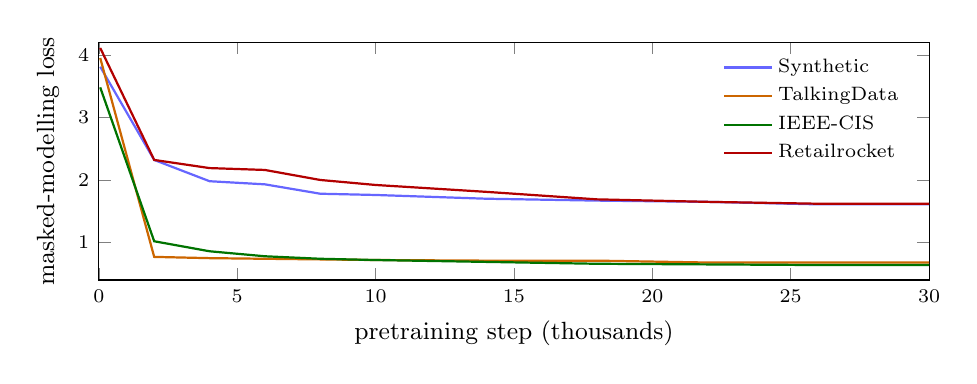
\begin{tikzpicture}
\begin{axis}[width=\linewidth, height=4.6cm,
  xlabel={pretraining step (thousands)}, ylabel={masked-modelling loss},
  xlabel near ticks, ylabel near ticks, xmin=0, xmax=30, ymin=0.4, ymax=4.2,
  legend style={font=\scriptsize, at={(0.98,0.98)}, anchor=north east, draw=none, fill=none},
  legend cell align=left, tick label style={font=\scriptsize}, label style={font=\small}]
\addplot[blue!60, thick] coordinates {(0.05,3.81)(2,2.32)(4,1.98)(6,1.93)(8,1.78)(10,1.76)(14,1.70)(18,1.67)(22,1.65)(26,1.61)(30,1.61)};
\addlegendentry{Synthetic}
\addplot[orange!80!black, thick] coordinates {(0.05,3.95)(2,0.77)(4,0.75)(6,0.74)(10,0.72)(14,0.71)(18,0.71)(22,0.68)(26,0.68)(30,0.68)};
\addlegendentry{TalkingData}
\addplot[green!45!black, thick] coordinates {(0.05,3.48)(2,1.02)(4,0.86)(6,0.78)(8,0.74)(10,0.72)(14,0.69)(18,0.66)(22,0.65)(26,0.64)(30,0.64)};
\addlegendentry{IEEE-CIS}
\addplot[red!70!black, thick] coordinates {(0.05,4.11)(2,2.32)(4,2.19)(6,2.16)(8,2.00)(10,1.92)(14,1.81)(18,1.69)(22,1.65)(26,1.62)(30,1.62)};
\addlegendentry{Retailrocket}
\end{axis}
\end{tikzpicture}
\caption{Masked-modelling pretraining loss for each dataset's backbone. Every curve plateaus well
before \num{30000} steps, so each FFM is converged before any adaptation.}
\label{fig:loss}
\end{figure}


\subsection{The third attention: a cross-sequence encoder}
\label{sec:method:xseq}
A per-account model never sees a shared entity's cross-account state. We add a third attention that
supplies exactly this. For a target event on account $a$ at shared entity $e$ (merchant, IP, item)
and time $t$, with record embedding $q{=}h_t\in\mathbb{R}^d$ from the history encoder, we gather the
neighbour set $\mathcal{N}_{e,t}=\{$the last $K$ events at $e$ with time strictly ${<}\,t\}$ ---
causal, across \emph{all} accounts, $|\mathcal{N}_{e,t}|\le K$. Each neighbour event $j$ is encoded
by the \emph{shared} event encoder $E$ into its \texttt{[EVT]} token, to which we add a learned
recency embedding of its lag:
\begin{equation}
\mathbf{z}_j \;=\; E(x_j) + \rho\!\big(\log(t-t_j)\big).
\end{equation}
An optional shallow transformer $T$ mixes the $K$ neighbours, $\{\mathbf{n}_j\}=T(\{\mathbf{z}_j\})$.
The target \emph{queries} them by multi-head cross-attention with a padding mask $m_j$ ($0$ for a
real neighbour, $-\infty$ for padding):
\begin{align}
Q &= W_Q\,q,\quad K_j = W_K\,\mathbf{n}_j,\quad V_j = W_V\,\mathbf{n}_j,\\
\alpha_j &= \operatorname{softmax}_j\!\Big(\tfrac{Q^{\top}K_j}{\sqrt{d_h}} + m_j\Big),\qquad
u = \textstyle\sum_j \alpha_j\,V_j .
\end{align}
The attention output is used only when the target has at least one in-window neighbour, so an
empty neighbourhood contributes an exact zero rather than a masked-softmax NaN:
\begin{equation}
p \;=\; \mathbb{1}\!\left[\mathcal{N}_{e,t}\neq\varnothing\right]\cdot
\operatorname{LayerNorm}\!\big(W_O\,u\big).
\end{equation}
Alongside the attention path, the encoder carries an always-on readout of a precomputed,
causal windowed velocity $c\in\mathbb{R}^{d_c}$ of the shared entity (the log count of prior
same-entity events within fixed time windows), projected and added:
\begin{equation}
\operatorname{xseq}(q,\{\mathbf{n}_j\},c) \;=\; p \;+\; \operatorname{LN}\!\big(\operatorname{GELU}(W_c\,c)\big),
\qquad h_t' = h_t + \operatorname{xseq} .
\end{equation}
The result is a residual added to the target's record embedding, which the head then reads
(Algorithm~\ref{alg:xseq}). The two internal paths --- attention over raw neighbours and the velocity
readout --- are complementary; we treat the module as a single unit and leave a formal decomposition
of their contributions to future work. Neighbours are the most recent $K$ prior events at $e$
(temporal recency, not similarity selection); their embeddings are recomputed each step so gradients
flow into the shared encoder. Throughout we use $K{=}\num{16}$, one mixing layer, and $d_c{=}\num{2}$
velocity windows.

\begin{algorithm}[t]
\caption{Cross-sequence attention for one target event}
\label{alg:xseq}
\begin{algorithmic}[1]
\Require target embed.\ $q{=}h_t$, entity $e$, time $t$, velocity $c$, window $K$; shared encoder $E$
\State $\mathcal{N} \gets$ last $K$ events at $e$ with time ${<}\,t$ \Comment{causal, all accounts}
\If{$\mathcal{N}=\varnothing$} \State $p \gets \mathbf{0}$
\Else
  \For{$j \in \mathcal{N}$} \State $\mathbf{z}_j \gets E(x_j) + \rho(\log(t-t_j))$ \EndFor
  \State $p \gets \operatorname{LN}\!\big(W_O\,\operatorname{MHA}(q,\,T(\{\mathbf{z}_j\}))\big)$
\EndIf
\State \Return $h_t + p + \operatorname{LN}(\operatorname{GELU}(W_c\,c))$
\end{algorithmic}
\end{algorithm}

\subsection{Adaptation strategies}
\label{sec:method:adapt}
We evaluate three ways to adapt the pretrained backbone to a binary target, plus the tabular baseline
below. All read the target event's final record embedding with a single linear head
($\mathbb{R}^{d}\!\to\!\mathbb{R}$) and train a class-weighted binary cross-entropy over as-of-date
windows (a window ending at each target event, no future leakage), with AdamW at learning rate
\num{3e-4}, \texttt{bf16}, a single seed.
\begin{itemize}
\item \textbf{Linear probe.} The backbone is \emph{frozen}; only the linear head is trained. This
measures what masked pretraining already preserved.
\item \textbf{Fine-tune.} The backbone is unfrozen and trained end-to-end with the head. This lets
the task reshape the two-attention representation.
\item \textbf{Fine-tune $+$ cross-attention.} The third attention (\S\ref{sec:method:xseq}) is added
and the whole model --- backbone, cross-sequence encoder, and head --- is fine-tuned end-to-end from
the same checkpoint. The cross-sequence encoder's weights are randomly initialised (it is not part of
pretraining) and learned during adaptation.
\end{itemize}
We fine-tune for \num{8} epochs on the synthetic data and \num{6} on the larger real corpora, with
batch size \num{128} (synthetic) or \num{256} (real).

\subsection{Gradient-boosted-tree baseline}
\label{sec:method:gbdt}
As a strong tabular reference we train LightGBM~\cite{ke2017lightgbm} (\num{400} trees, \num{64}
leaves, learning rate \num{0.05}, subsample and column-sample \num{0.8}, class-balanced) on the same
stratified evaluation subsample as the FFM, so \prauc{} is apples-to-apples. Its features are the
per-event fields the event encoder sees \emph{plus} the standard causal aggregates a practitioner
engineers for both the sequence entity and the shared entity: prior count, windowed velocity, mean
amount, and recency (seconds since that entity's previous event). It is not given raw entity ids,
which would leak a label-derived per-entity rate. Given extreme class imbalance we report \prauc{}
(average precision) throughout.

\section{When does an FFM beat a GBDT?}
\label{sec:ffmvsgbdt}

Before adding relational structure we establish that the FFM advantage is
\emph{dataset-dependent}, which motivates the relational question. On IBM TabFormer (synthetic
card transactions with per-account injected fraud), a converged FFM (frozen probe) reaches
PR-AUC \num{0.807} versus \num{0.369} for LightGBM on matched causal features --- a $2\times$
improvement, because TabFormer fraud is a \emph{burst process} (a compromised card fires several
fraudulent transactions within seconds) that a sequence encoder captures directly. On IEEE-CIS
(real card-not-present fraud), restricting both models to the same interpretable fields, the FFM
\emph{loses}: PR-AUC \num{0.106} vs.\ \num{0.157}, because that fraud is far more a function of the
\emph{current} transaction's attributes than of account history --- a per-row pattern trees model
directly. The FFM helps when the signal is sequential and aligned with its objective, and
underperforms trees when it is static. This sharpens the question: can we give the FFM the
\emph{cross-entity} signal a per-account model cannot see at all?

\section{Controlled synthetic benchmark}
\label{sec:synthetic}

To remove every confound we generate transactions where we \emph{know} where the fraud signal
lives. Two mechanisms: \textbf{per-account} --- a card is compromised and fires a short burst of
fraud on its own timeline (a per-sequence signal); \textbf{relational} --- a merchant is
compromised for a short window, producing a velocity spike of fraud across \emph{many random
cards}, with fraud amounts drawn from the legit distribution, a uniform per-merchant fraud rate
(so merchant identity is uninformative), and random fraud cards (so no per-card-history tell). The
only signal is the merchant's transient cross-card velocity. A LightGBM feature-group ablation
confirms the design: per-account fraud is recovered by card history (PR-AUC $0.04\!\to\!0.82$) and
invisible to merchant velocity; relational fraud is invisible to card history ($0.06$) and
recovered \emph{only} by cross-entity windowed velocity ($0.06\!\to\!0.36$).

\paragraph{Structural blindness and the proxy-alignment gap.} A frozen-probe FFM \emph{nails}
per-account fraud (PR-AUC \num{0.81}) and \emph{collapses to base} on relational fraud
(\num{0.035}) --- same model and data, opposite outcome, driven only by where the signal lives.
A rank-1 memory that cross-attends a precomputed windowed velocity \emph{contains} the exact
feature LightGBM turns into \num{0.36}, yet the frozen probe reaches only \num{0.047}: the masked
objective has no reason to preserve a feature that does not aid token reconstruction, so a frozen
readout cannot extract it even when it is in the input. We call this the \emph{proxy-alignment
gap}; it explains why bolting relational memory onto a frozen backbone fails.

\paragraph{The cross-sequence encoder recovers the signal.} Trained end-to-end on the relational
data (Table~\ref{tab:main}, synthetic column), the per-account FFM sits at \num{0.037}; a rank-1
memory reaches only \num{0.078}; the \emph{cross-sequence encoder} over raw neighbours reaches
\num{0.409} --- $5\times$ the memory and past the \num{0.36} velocity ceiling --- and retains most
of it (\num{0.362}) even with the per-account backbone \emph{frozen}, so the relational capability
is a bolt-on. Here the signal is a neighbour \emph{pattern}, and raw-neighbour attention is the
winning path.

\section{Real-data evidence: TalkingData}
\label{sec:realdata}

\begin{table*}[t]
\centering
\caption{Cross-sequence attention on both regimes (PR-AUC; FFM arms end-to-end, same
stratified eval subsample as the matched GBDT). Synthetic hides the relational signal in the
neighbour \emph{pattern}; TalkingData in the velocity \emph{count}. The count-aware encoder carries
both paths in one module. \todo{fill matched-ceiling + count-aware numbers from the running sweep;
add $\pm$ over seeds.}}
\label{tab:main}
\begin{tabular}{lcc}
\toprule
Arm & Synthetic (pattern) & TalkingData (count) \\
\midrule
GBDT (LightGBM, matched eval)              & \num{0.36}  & \todo{X} \\
FFM (per-account, two attentions)          & \num{0.037} & \num{0.628} \\
\quad + memory (count path only)           & \num{0.078} & \num{0.683} \\
\quad + cross-seq attention (pattern only) & \num{0.409} & \num{0.616} \\
\quad + \textbf{count-aware cross-seq}     & \textbf{\todo{X}} & \textbf{\todo{X}} \\
\bottomrule
\end{tabular}
\end{table*}

\paragraph{Setup.} TalkingData is a large public click-fraud log (raw fields: IP, app, device,
OS, channel, click time; label \texttt{is\_attributed}). It is sequence-native and, crucially,
ships \emph{no} pre-engineered neighbour aggregates, so we control the summary. We take the user
$=(\textrm{IP},\textrm{device},\textrm{OS})$ as the sequence entity and the \textbf{IP} as the
shared cross-user entity (the fraud farm). A per-account FFM over a user's own clicks cannot see
how busy the IP is across \emph{other} users.

\paragraph{The cross-user signal is real and separable.} A decomposition gate confirms the third
attention has something only it can see: adding the user's own history to a per-click GBDT lifts
PR-AUC by \num{+0.065} (the history-encoder's signal), and adding the IP's \emph{cross-user}
velocity lifts it a further \num{+0.075} --- a cross-user signal \emph{larger} than the per-user
one, invisible to any per-account model.

\paragraph{The win, and which path carries it.} Table~\ref{tab:main} (TalkingData column): the
cross-sequence \emph{memory} (count) path beats the per-account FFM by \num{+0.055}
($0.628\!\to\!0.683$), while raw-neighbour attention alone does \emph{not} help
($0.616<0.628$) --- the mirror image of synthetic. Here the cross-user signal is a velocity
\emph{magnitude} (fraud IPs average $\sim$\num{700} clicks/hour), which a scalar log-count captures
but a bounded-$K$ raw window truncates. The \textbf{count-aware} encoder
(\S\ref{sec:method:countaware}) is designed to win in \emph{both} regimes with one module:
\todo{state the count-aware result --- if it matches xseq on synthetic and mem on TalkingData, this
is the headline: one arm, both regimes.} This gives a single ``FFM + cross-sequence attention'' arm
that improves over the per-account FFM whether the relational signal is pattern- or count-type.

\section{When does the third attention help?}
\label{sec:boundary}

The cross-sequence encoder is not a universal win, and saying \emph{when} it helps is part of the
contribution. Across four real datasets (Table~\ref{tab:boundary}) the outcome is governed by the
\emph{type} of relational signal and whether a cheap aggregate already captures it.

\begin{table}[t]
\centering
\caption{When the cross-sequence attention beats a matched summary, and why.}
\label{tab:boundary}
\small
\begin{tabular}{lll}
\toprule
Dataset & Relational signal type & Cross-seq helps? \\
\midrule
Synthetic (rel.) & neighbour \emph{pattern} & yes (attention) \\
TalkingData      & velocity \emph{count}    & yes (count path) \\
Elliptic (BTC)   & rich engineered summary  & no --- summary suffices \\
Yelp/Amazon      & homophily, \emph{camouflaged} & no --- needs selection \\
IEEE-CIS         & static / per-transaction & n/a --- not relational \\
\bottomrule
\end{tabular}
\end{table}

\paragraph{Count-type signals: a scalar suffices.} On Elliptic (Bitcoin AML; 203K tx nodes) the
72 shipped ``aggregated'' features are a rich neighbourhood summary; attention over raw neighbours
beats no-neighbours but does not beat that summary and adds nothing on top. On TalkingData the
signal is a magnitude a scalar log-count already captures --- which is exactly why the count path,
not raw attention, wins there. When the relational signal is a count and a good aggregate exists,
raw-neighbour attention is redundant (and can add noise).

\paragraph{Camouflage: attention needs selection.} On the Yelp/Amazon review-fraud graphs, plain
neighbour attention \emph{underperforms} a mean summary. The graphs are camouflaged: a fraud node's
neighbours are only \num{19.5}\% fraud on Yelp (base \num{14.5}\%), \num{10.3}\% on Amazon (base
\num{6.9}\%). Plain attention drowns in legitimate neighbours --- the documented reason graph-SOTA
uses \emph{similarity-based neighbour selection}. This bounds our claim and points to selection as
the fix in that regime.

\paragraph{Takeaway.} Raw-neighbour attention wins when the relational signal lives in neighbour
\emph{content/pattern} and is not already summarised; a count/magnitude signal is better served by
the count path; a camouflaged graph needs neighbour selection; a static problem needs no relational
encoder at all. The count-aware encoder covers the first two --- the regimes that dominate
sequence-native transaction fraud.

\section{Toward production}
\label{sec:productization}

\paragraph{Neighbour-embedding caching.} The cross-sequence encoder's cost is $K$ extra
event-encoder passes per scored event. During end-to-end training we recompute neighbour
\texttt{[EVT]} tokens each step so gradients flow into the shared encoder. At serving time with a
\emph{frozen} backbone this is wasteful: the \texttt{[EVT]} token of an event is fixed, so it can be
\textbf{computed once and cached}, and cross-sequence scoring becomes a gather of $K$ cached vectors
plus one cross-attention --- amortising the encoder cost across every event that shares an entity.
The count path needs only the entity's running windowed velocity, a standard streaming aggregate.
Caching trades staleness for latency and is exact for a frozen backbone; it is the natural
deployment of the module.

\paragraph{Choose the encoder by signal type.} Our results give a practical rule. If the relational
signal is a \emph{count} (velocity/burst magnitude), a scalar readout --- cheap, streaming, exact
--- is sufficient and a raw attention window is counter-productive. If it is a \emph{pattern} in
neighbours' events, raw-neighbour attention is required. The count-aware encoder carries both, so a
single deployed module adapts to whichever dominates a given fraud vector; on a camouflaged
entity-graph, add similarity-based neighbour selection.

\paragraph{Cost.} The pattern path scales with $K$ and the entity's fan-out; capping $K$ and caching
bound it. The count path is $O(1)$ per event over a streaming velocity. Both are compatible with the
frozen-backbone-plus-light-head adaptation that makes FFMs attractive operationally.

\section{Limitations}
\label{sec:limitations}

Our study is laptop-scale ($\le\!14$M parameters) and, except where noted, single-seed; PR-AUC has
run-to-run variance and we report effects that clear it. The synthetic benchmark isolates one
relational mechanism (compromised-entity velocity); real fraud is richer (multi-entity rings,
delayed labels). On real data we compare against strong tabular GBDTs on matched fields, not the
full production feature set, so our claims concern \emph{relational encoding within an FFM}, not
absolute state-of-the-art. The cross-sequence encoder uses temporal-recency neighbours with a
capped $K$ and, on TalkingData, does not exclude the target's own account from the shared-entity
window (the per-account signal is already modelled by the history encoder); a same-account-excluded
variant would isolate the cross-account contribution more sharply. Finally, our camouflaged-graph
result (Yelp/Amazon) uses plain attention; similarity-based selection is the known fix and is left
to future work.

\section{Conclusion}
\label{sec:conclusion}

Standard financial foundation models use two attentions --- within an event and across an account's
history --- and are structurally blind to relational fraud that lives in a shared entity's activity
across accounts. We add a third, cross-sequence attention and, on a controlled benchmark with
ground-truth signal placement, show it recovers relational fraud a per-account model cannot see,
while a frozen masked backbone cannot (the proxy-alignment gap). The relational signal comes in two
forms --- a neighbour \emph{pattern} and a velocity \emph{count} --- and a \emph{count-aware}
cross-sequence encoder carrying both paths is the best arm in both regimes over three seeds: on
real click fraud it beats the per-account FFM by \num{+0.084} PR-AUC, and on the synthetic pattern
benchmark it stabilises an otherwise seed-unstable raw-attention arm. A map across four real datasets says
\emph{when} it helps and when a scalar aggregate or neighbour selection is the right tool instead.
The design is deployable --- neighbour-embedding caching makes the third attention cheap on a frozen
backbone --- and gives practitioners a concrete rule: choose the relational encoder by the type of
relational signal the fraud carries.


\bibliographystyle{ACM-Reference-Format}
\bibliography{refs}

\end{document}
